\begin{questions}
\question
In the figure below, the two squares are translating horizontally in the opposite directions as indicated by the arrows. Indicate the respective perceived motions if you are looking through the apertures 1, 2, and 3. Explain your answers.

\begin{figure}[H]
    \centering
    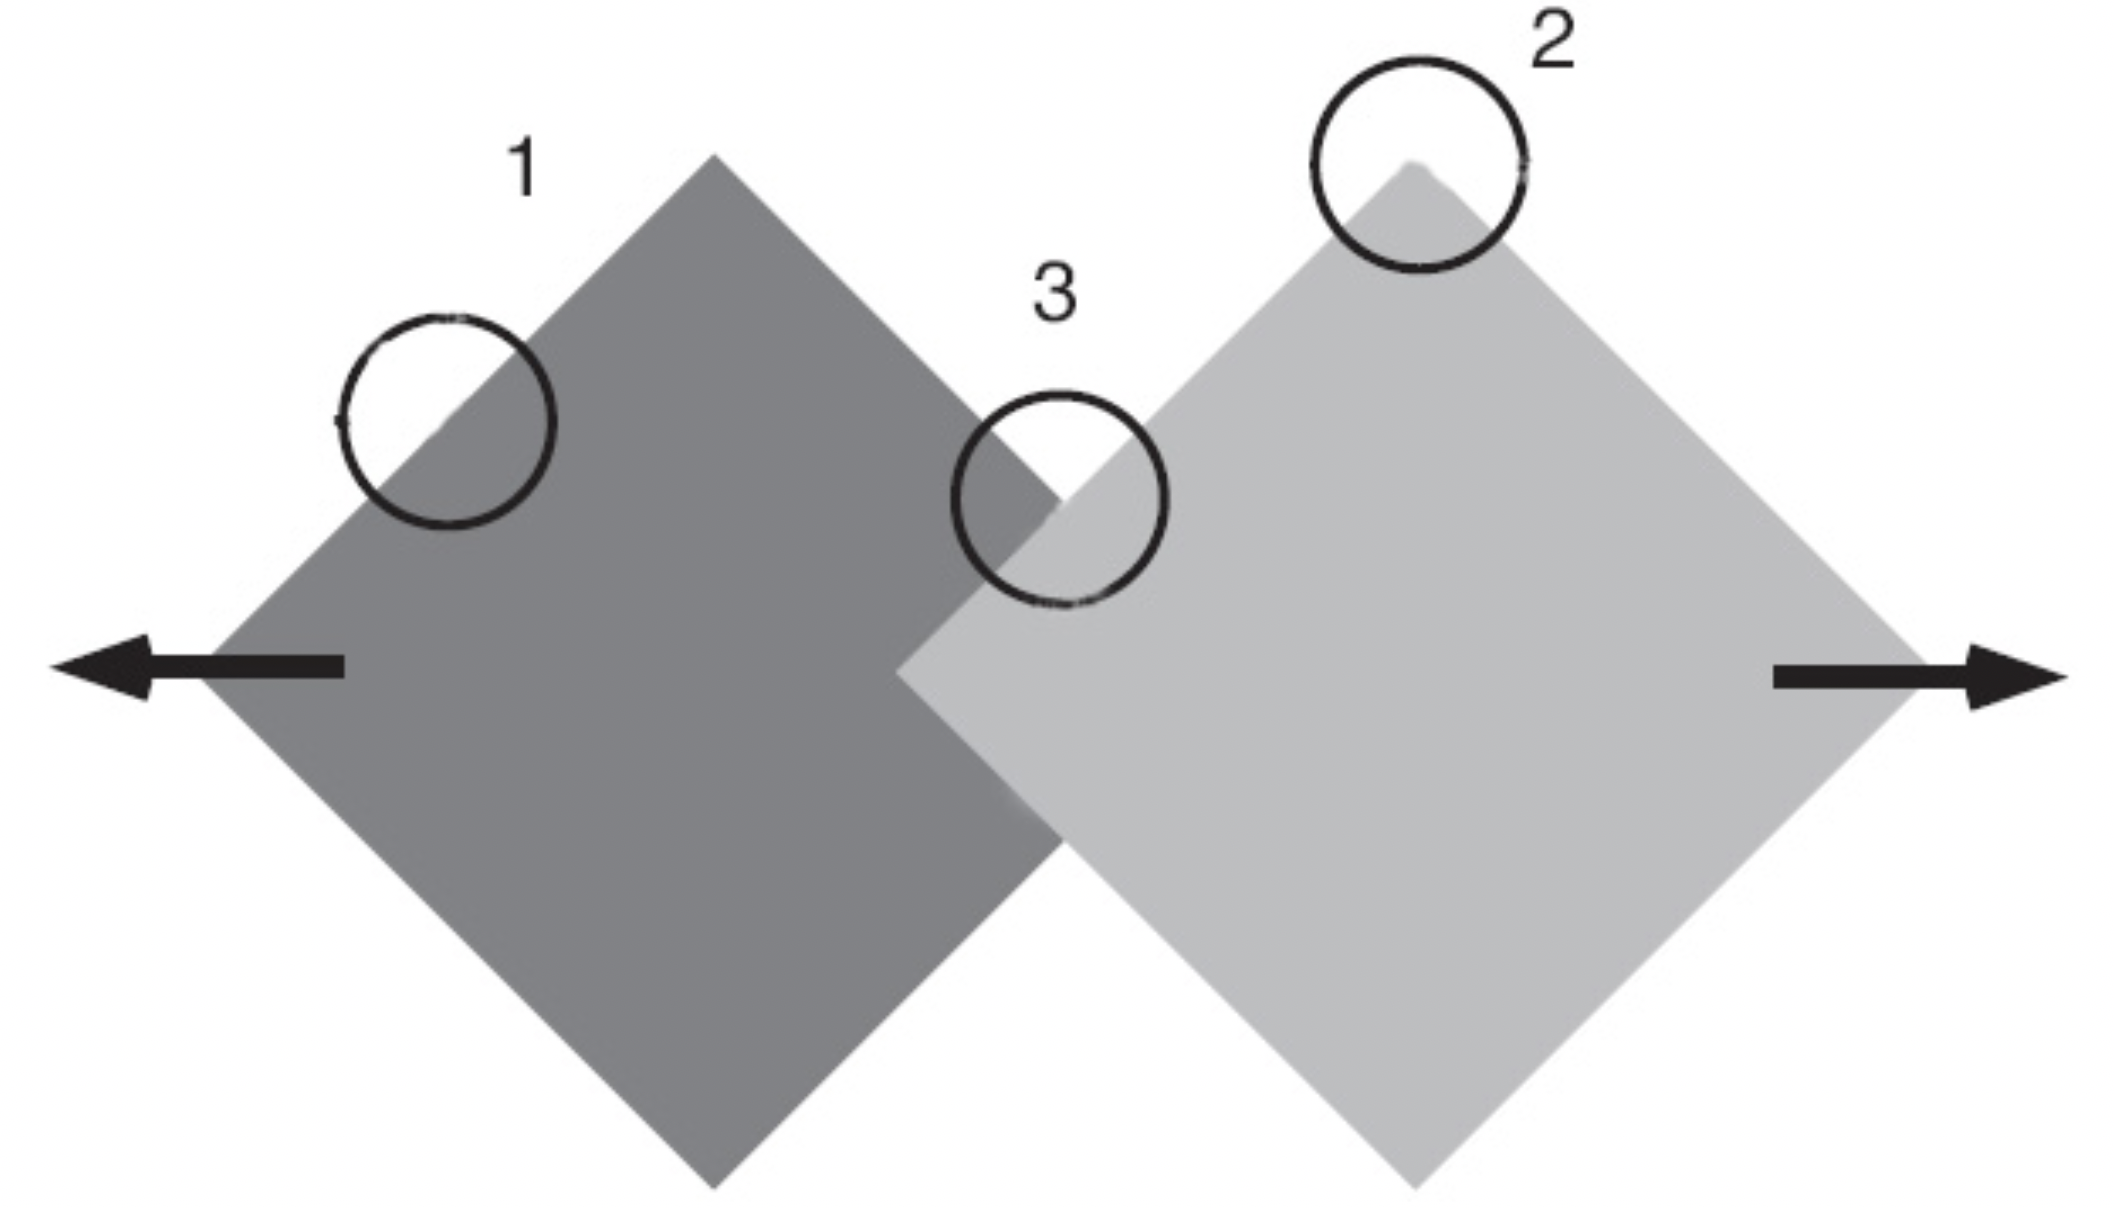
\includegraphics[width=0.6\linewidth]{square_motion.png}
    \caption{Two squares translating horizontally in the opposite directions.}
\end{figure}

\begin{solution}
    Based on Brightness Constancy Equation assumption, we humans can observe the normal flow of an object within an aperture.\\
    Donald Hoffman has explained this ``aperture problem" as the choice of our visual system to construct the smallest motion. This choice is motion orthogonal to the line that moves \cite{HD}.\\
    At \textbf{aperture 1}, the perceived motion will be pointing to the upper left direction that is perpendicular to the edge. This is because without context, we can only see the movement of the edge (the sharp change of intensity) and conclude that the object is moving perpendicular to its edge.\\
    At \textbf{aperture 2}, the perceived motion will be pointing vertically downwards, with the assumption that the two squares are moving with the same speed in the opposite direction. Due to symmetry, the corner formed by two edges of two squares will moving downwards. And because of it, we will perceive that the object is moving downwards since the corner is the motion clue we can see through this aperture.\\
    At \textbf{aperture 3}, the perceived motion will be pointing to the right. The reason is similar to aperture 2, with the corner giving us clues about the object's motion.
\end{solution}

\question
Barber-pole with Occlusion: The figure below illustrates various barber-pole configurations, with occluders placed along either vertical or horizontal sides of the barber-pole. The arrows indicate the perceived direction of barber-pole motion. Explain why the perceived motion tends to be biased in the direction orthogonal to the occlusion boundary.

\begin{figure}[H]
    \centering
    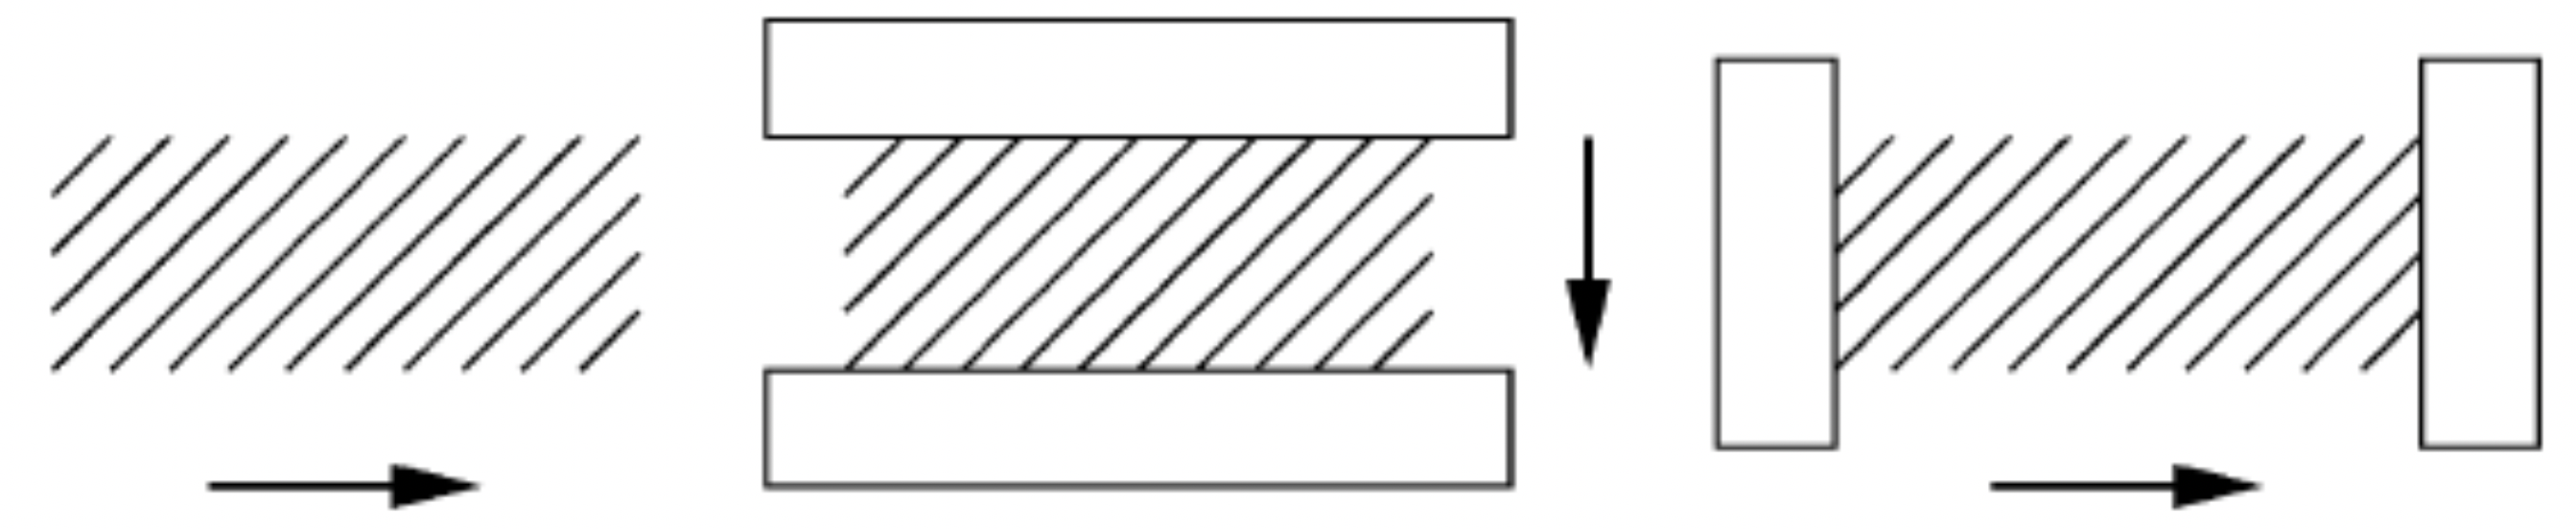
\includegraphics[width=0.6\linewidth]{Barber_pole.png}
    \caption{Barber-pole with occlusion. Arrows indicate the perceived motion. Left: Barber-pole with no occluders. Middle: Occluders placed on the top and bottom cause the perceived motion to be mostly vertical. Right: Occluders placed on the left and right sides of the barber-pole bias the perceived motion toward horizontal.}
\end{figure}

\begin{solution}
    For a barber-pole, the diagonally oriented lines are spinning inside the occluder. However, he eyes use the visual cues where the stripes end at the sides of the pole to override any visual depth cues, and therefore the stripes appear to move vertically or horizontally rather than spin. \\
    In addition, the line terminators aligned with the occluders are considered as \textbf{extrinsic} terminators, therefore their motion signals tend to
    become more ambiguous and have less influence on the perceived motion \cite{vis04}. This is the reason for perceiving the middle scenario as moving downwards. And for the right scenario, it is obvious that more number of intrinsic terminators are moving horizontally so that we perceive it moving rightwards. 
\end{solution}

\question
* Referring to the diagram below, the stimulus consists of two orthogonal bars that move sinusoidally, 90 degree out of phase (Figure a and b). When presented together within an occluding aperture (Figure c), the bars perceptually cohere and appear to move in a circle as a solid cross. However, when presented alone (Figure d), they appear to move separately (the horizontal bar translates vertically and the vertical bar translates horizontally), even though the image motion is unchanged in Figures c and d. In either stimulus condition, both percepts are legitimate interpretations of the image motion. Yet a single interpretation is predominantly seen in each case. Why?

\begin{figure}[H]
    \centering
    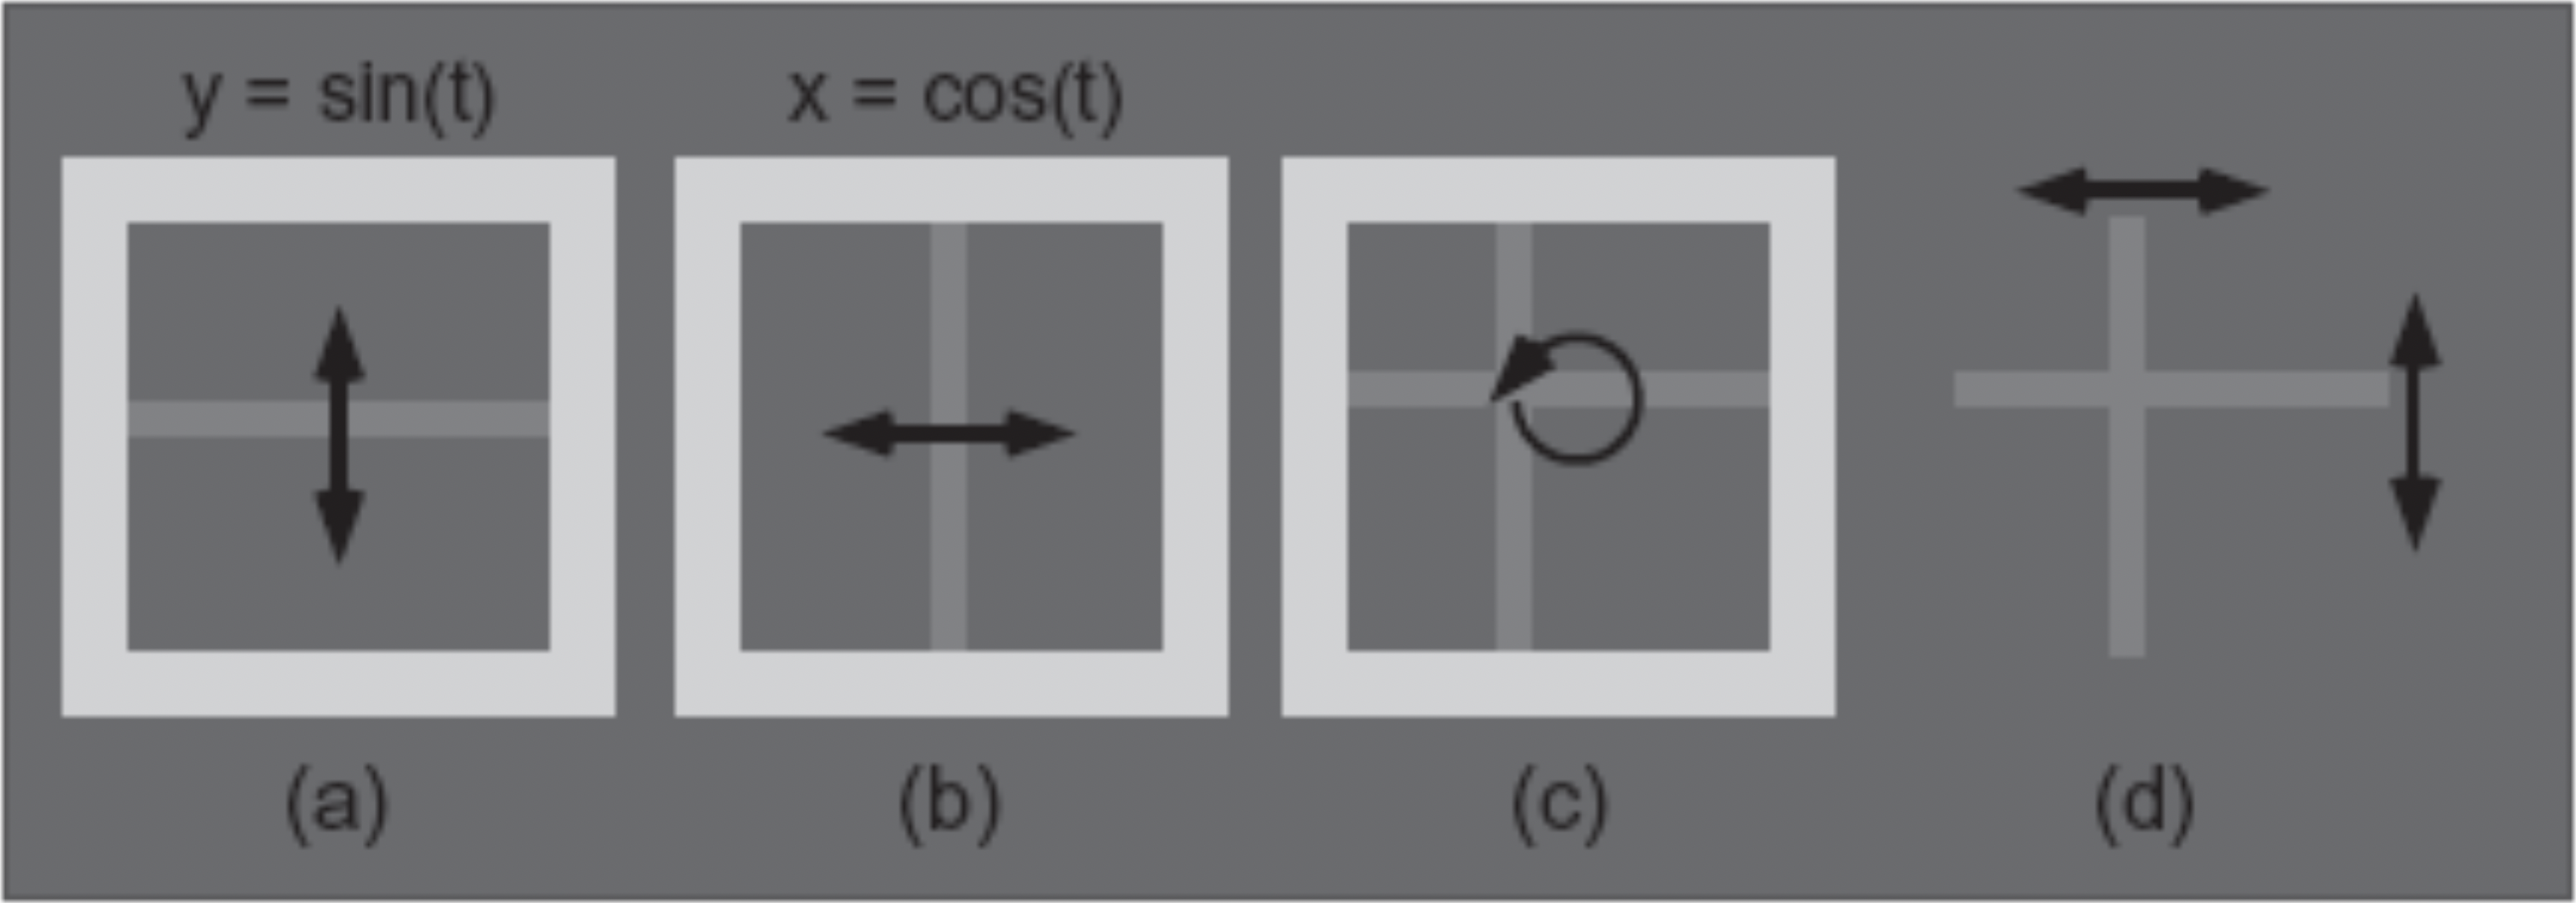
\includegraphics[width=0.6\linewidth]{stimulus.png}
\end{figure}

\begin{solution}
    In the configuration (d), the bar endpoints are clearly seen by viewers. It can provide unambiguous two dimensional motion signals, which are believed to determine the motion percept. The endpoints move linearly, and each bar follows along.\\
    However, when the frame is present, the T-junctions are formed at the bar endpoints. These junctions provide a cue that the endpoint motions are the spurious result of occlusion. Thus, the motion at T-junctions will have less influence on our perception. With this, the circular motion of the bar intersection determines the motion percept, as all the local motions in the stimulus apart from those of the endpoints are consistent with such a circular motion.
\end{solution}

\question
* For a purely rotational motion, the equation that relates the optical flow $(u, v)$ to its rotational parameters $(\omega_{x}, \omega_{y}, \omega_{z})$ is of the conic form explored in Questions $3d$ and $3e$:
\begin{equation}
        \begin{aligned} u &=\omega_{x} x y-\omega_{y}\left(x^{2}+1\right)+\omega_{z} y \\ v &=\omega_{x}\left(y^{2}+1\right)-\omega_{y} x y-\omega_{z} x \end{aligned}
\end{equation}
Assume you are given enough optical flow measurements at different $(x, y)$ locations, solve $(\omega _ {x}, \omega _ {y}, \omega _ {z})$ in the least squares sense by writing down the least squares equation of the form $Ax=b, (b \neq 0)$. Explain why in this case, the equation is of the non-homogeneous form, whereas that in Question 3e is of the homogeneous form $Ax=0$, and explain whether it is appropriate or inappropriate to change the formulation of this question to the $Ax=0$ form.

\begin{solution}
    The least squares equation is formed as:
    \begin{equation}
        \begin{bmatrix}
            xy & -(x^{2} + 1) & y \\
            y ^ {2} + 1 & -xy & -x
        \end{bmatrix}
        \left( \begin{array}{c}
           \omega _ {x} \\  
           \omega _ {y} \\  
           \omega _ {z} \\  
        \end{array}\right) = \left(\begin{array}{c}
             u \\
             v
        \end{array}\right)
    \end{equation}
    In this question, there are three unknowns and two equations. The matrix is rank-deficient and thus we'd like to use SVD and compute the psedo-inverse. It is not suitable to change to $Ax=0$ (homogeneous) form because the null vector will not be unique. But in question 3e, which is an over-determined question, we just take the eigenvector of $A^{T}A$ corresponding to the smallest singular value.
    
\end{solution}
    


\end{questions}
    




